\documentclass[a4paper,11pt,fleqn,twoside,notitlepage]{report}
\usepackage[]{graphicx}\usepackage[]{color}
%% maxwidth is the original width if it is less than linewidth
%% otherwise use linewidth (to make sure the graphics do not exceed the margin)
\makeatletter
\def\maxwidth{ %
  \ifdim\Gin@nat@width>\linewidth
    \linewidth
  \else
    \Gin@nat@width
  \fi
}
\makeatother

\definecolor{fgcolor}{rgb}{0.345, 0.345, 0.345}
\newcommand{\hlnum}[1]{\textcolor[rgb]{0.686,0.059,0.569}{#1}}%
\newcommand{\hlstr}[1]{\textcolor[rgb]{0.192,0.494,0.8}{#1}}%
\newcommand{\hlcom}[1]{\textcolor[rgb]{0.678,0.584,0.686}{\textit{#1}}}%
\newcommand{\hlopt}[1]{\textcolor[rgb]{0,0,0}{#1}}%
\newcommand{\hlstd}[1]{\textcolor[rgb]{0.345,0.345,0.345}{#1}}%
\newcommand{\hlkwa}[1]{\textcolor[rgb]{0.161,0.373,0.58}{\textbf{#1}}}%
\newcommand{\hlkwb}[1]{\textcolor[rgb]{0.69,0.353,0.396}{#1}}%
\newcommand{\hlkwc}[1]{\textcolor[rgb]{0.333,0.667,0.333}{#1}}%
\newcommand{\hlkwd}[1]{\textcolor[rgb]{0.737,0.353,0.396}{\textbf{#1}}}%

\usepackage{framed}
\makeatletter
\newenvironment{kframe}{%
 \def\at@end@of@kframe{}%
 \ifinner\ifhmode%
  \def\at@end@of@kframe{\end{minipage}}%
  \begin{minipage}{\columnwidth}%
 \fi\fi%
 \def\FrameCommand##1{\hskip\@totalleftmargin \hskip-\fboxsep
 \colorbox{shadecolor}{##1}\hskip-\fboxsep
     % There is no \\@totalrightmargin, so:
     \hskip-\linewidth \hskip-\@totalleftmargin \hskip\columnwidth}%
 \MakeFramed {\advance\hsize-\width
   \@totalleftmargin\z@ \linewidth\hsize
   \@setminipage}}%
 {\par\unskip\endMakeFramed%
 \at@end@of@kframe}
\makeatother

\definecolor{shadecolor}{rgb}{.97, .97, .97}
\definecolor{messagecolor}{rgb}{0, 0, 0}
\definecolor{warningcolor}{rgb}{1, 0, 1}
\definecolor{errorcolor}{rgb}{1, 0, 0}
\newenvironment{knitrout}{}{} % an empty environment to be redefined in TeX

\usepackage{alltt}
\newcommand{\SweaveOpts}[1]{}  % do not interfere with LaTeX
\newcommand{\SweaveInput}[1]{} % because they are not real TeX commands
\newcommand{\Sexpr}[1]{}       % will only be parsed by R


\setcounter{tocdepth}{3}
\setcounter{secnumdepth}{3}

\usepackage[utf8]{inputenc}
\usepackage[margin=2.5cm]{geometry}
\usepackage{graphicx}
\usepackage[T1]{fontenc}
\usepackage{enumitem}
\usepackage[section]{placeins}
\usepackage{csquotes}
\usepackage[english]{babel}
\usepackage{float}
\usepackage{caption}
\usepackage{makecell}
\usepackage{hyperref}
\usepackage{bm}
\usepackage{newfloat}
\usepackage[linesnumbered,lined,boxed,commentsnumbered]{algorithm2e}
\usepackage{booktabs}
\usepackage{colortbl}
\usepackage{tikz}

\usepackage{amssymb,amsmath,amsthm,amsfonts}
\newtheorem{theorem}{Theorem}

\usepackage{fancyhdr}
\setlength{\headheight}{15pt}

\pagestyle{fancy}
\renewcommand{\chaptermark}[1]{ \markboth{#1}{} }
\renewcommand{\sectionmark}[1]{ \markright{#1}{} }

\fancyhf{}
\fancyfoot[CE,CO]{\thepage}
\fancyhead[LE]{\textit{ \nouppercase{\leftmark}} }
\fancyhead[LO]{\textit{ \nouppercase{\rightmark}} }
%\fancyhead[RE,RO]{Erik Thors\'{e}n, \href{mailto:Ethorsn@gmail.com}{Ethorsn@gmail.com} }
\fancypagestyle{plain}{ %
\fancyhf{} % remove everything
  \renewcommand{\headrulewidth}{0pt} % remove lines as well
  \renewcommand{\footrulewidth}{0pt}
}

\usepackage[citestyle=authoryear,natbib=true,backend=bibtex,hyperref=true,maxnames=1]{biblatex}

%\addbibresource{REFERENCES.bib}
\bibliography{REFERENCES.bib}

\title{Statistical process control in next-generation sequencing quality control data}
\author{Erik Thors\'{e}n \thanks{Postal adress: Mathematical Statistics, Stockholm University, SE-106 91, Sweden. E-mail: Ethorsn@gmail.com. Supervisors: Taras Bodnar and Johan Dahlberg}}
\date{\today}

\raggedbottom


\begin{document}


\begin{knitrout}
\definecolor{shadecolor}{rgb}{0.969, 0.969, 0.969}\color{fgcolor}\begin{kframe}
\begin{alltt}
\hlkwd{load}\hlstd{(}\hlstr{"../Data/WishartH.Rdata"}\hlstd{)}
\hlkwd{load}\hlstd{(}\hlstr{"../Data/meanH.Rdata"}\hlstd{)}
\hlkwd{load}\hlstd{(}\hlstr{"../Data/Case1Mean.Rdata"}\hlstd{)}
\hlkwd{load}\hlstd{(}\hlstr{"../Data/Case2Mean.Rdata"}\hlstd{)}
\hlkwd{load}\hlstd{(}\hlstr{"../Data/Case1Sigma.Rdata"}\hlstd{)}
\hlkwd{load}\hlstd{(}\hlstr{"../Data/Case2Sigma.Rdata"}\hlstd{)}
\hlkwd{load}\hlstd{(}\hlstr{"../Data/ICdata.Rdata"}\hlstd{)}
\hlkwd{load}\hlstd{(}\hlstr{"../Data/CPDsims.Rdata"}\hlstd{)}
\hlstd{M} \hlkwb{<-} \hlkwd{nrow}\hlstd{(TransformedData)}
\hlstd{p} \hlkwb{<-} \hlkwd{ncol}\hlstd{(TransformedData)}
\hlstd{alpha} \hlkwb{<-} \hlnum{0.01}

\hlstd{QuantileHot} \hlkwb{<-} \hlstd{p}\hlopt{*}\hlstd{(M}\hlopt{-}\hlnum{1}\hlstd{)}\hlopt{*}\hlstd{(M}\hlopt{+}\hlnum{1}\hlstd{)}\hlopt{/}\hlstd{((M}\hlopt{-}\hlstd{p)}\hlopt{*}\hlstd{M)} \hlopt{*} \hlkwd{qf}\hlstd{(}\hlnum{1}\hlopt{-}\hlstd{alpha, p, M}\hlopt{-}\hlstd{p)}

\hlstd{K} \hlkwb{<-} \hlnum{100}
\hlstd{OrgOrder} \hlkwb{<-} \hlkwd{colnames}\hlstd{(TransformedData)}
\hlcom{# divide by a constant!}
\hlstd{TransformedData[,}\hlnum{1}\hlopt{:}\hlkwd{ncol}\hlstd{(TransformedData)} \hlopt \hlkwd{grep}\hlstd{(}\hlstr{"mean"}\hlstd{,OrgOrder)]} \hlkwb{<-} \hlstd{TransformedData[,}\hlnum{1}\hlopt{:}\hlkwd{ncol}\hlstd{(TransformedData)} \hlopt \hlkwd{grep}\hlstd{(}\hlstr{"mean"}\hlstd{,OrgOrder)]}\hlopt{/}\hlstd{K}

\hlstd{mu0} \hlkwb{<-} \hlkwd{colMeans}\hlstd{(TransformedData)}
\hlstd{Sigma0} \hlkwb{<-} \hlkwd{var}\hlstd{(TransformedData)}\hlopt{*}\hlstd{(M}\hlopt{-}\hlnum{1}\hlstd{)}\hlopt{/}\hlstd{M}

\hlstd{Rcpp}\hlopt{::}\hlkwd{sourceCpp}\hlstd{(}\hlstr{"../FunctionsAndRcpp/RcppHotellingT2.cpp"}\hlstd{)}
\hlcom{###################### Found online function! webpage: http://www.sthda.com/english/wiki/ggplot2-easy-way-to-mix-multiple-graphs-on-the-same-page-r-software-and-data-visualization}
\hlstd{get_legend} \hlkwb{<-}\hlkwa{function}\hlstd{(}\hlkwc{myggplot}\hlstd{)\{}
  \hlstd{tmp} \hlkwb{<-} \hlkwd{ggplot_gtable}\hlstd{(}\hlkwd{ggplot_build}\hlstd{(myggplot))}
  \hlstd{leg} \hlkwb{<-} \hlkwd{which}\hlstd{(}\hlkwd{sapply}\hlstd{(tmp}\hlopt{$}\hlstd{grobs,} \hlkwa{function}\hlstd{(}\hlkwc{x}\hlstd{) x}\hlopt{$}\hlstd{name)} \hlopt{==} \hlstr{"guide-box"}\hlstd{)}
  \hlstd{legend} \hlkwb{<-} \hlstd{tmp}\hlopt{$}\hlstd{grobs[[leg]]}
  \hlkwd{return}\hlstd{(legend)}
\hlstd{\}}
\hlcom{#######################}
\end{alltt}
\end{kframe}
\end{knitrout}
\section{Calculation of control limits}
The number of variables is equal to $p=48$ and the number of observation in the IC sample is equal to $M=73$. Using $\alpha=0.01$, the control limit of Hotelling's $T^2$ is equal to $337.57$. 

To calculate the control limits for the MCUSUM scheme we use the function \texttt{CalculateControlLimit}, described in section \ref{AVERG}. In this thesis we will use a set of allowance constants $k$ to see how the different control charts act with the use of different allowance constants. The following inputs was used in the calculations of the control limits.
\begin{itemize}
\item Allowance constants $k = \{0.30, 0.40, 0.50\}.$
\item Target in-control average run length ARL$^*_0 = 100$.
\item Maximum number of iterations Nmax= 40 or 20.
\item The number $\epsilon$ was set to $0.05$.
\item The number of simulations was set to $10^5$ 
\end{itemize}
The in-control parameters $\boldsymbol{\mu}_0$ and $\boldsymbol{\Sigma}_0}$ were estimated from the transformed data. The constant $a_0$ was set sufficiently small in each simulation to ensure convergence, often close or equal to zero. The upper limit $b_0$ was tailored for each allowance constant, $k$. For $k=0.3$, $b_0$ was chosen large, equal to $1000$ or $10 000$ since no prior information on the control limit is available. In the next calculation with a larger allowance constant $k$, $b_0$ was chosen close to the calculated control limit in previous step with a smaller allowance constant. In Table \ref{Control} the control limits are listed for the mean and covairance chart with the use of different allowance constants. 
\begin{kframe}
\begin{alltt}
\hlstd{k} \hlkwb{<-} \hlkwd{c}\hlstd{(}\hlnum{0.3}\hlstd{,}\hlnum{0.4}\hlstd{,}\hlnum{0.5}\hlstd{)}
\hlkwd{library}\hlstd{(dplyr)}
\end{alltt}


{\ttfamily\noindent\itshape\color{messagecolor}{\#\# \\\#\# Attaching package: 'dplyr'}}

{\ttfamily\noindent\itshape\color{messagecolor}{\#\# The following objects are masked from 'package:stats':\\\#\# \\\#\#\ \ \ \  filter, lag}}

{\ttfamily\noindent\itshape\color{messagecolor}{\#\# The following objects are masked from 'package:base':\\\#\# \\\#\#\ \ \ \  intersect, setdiff, setequal, union}}\begin{alltt}
\hlkwd{library}\hlstd{(grid)}

\hlstd{Control.Limits.mean} \hlkwb{<-} \hlkwd{lapply}\hlstd{(H_Listmean,} \hlkwa{function}\hlstd{(}\hlkwc{x}\hlstd{) x}\hlopt{$}\hlstd{Intervals} \hlopt
  \hlkwd{na.omit}\hlstd{()} \hlopt
  \hlkwd{tail}\hlstd{(}\hlnum{1}\hlstd{)} \hlopt
  \hlkwd{mean}\hlstd{())} \hlopt
  \hlkwd{unlist}\hlstd{()} \hlopt
  \hlkwd{round}\hlstd{(}\hlnum{3}\hlstd{)}

\hlstd{Control.Limits.Cov} \hlkwb{<-} \hlkwd{lapply}\hlstd{(H_ListSigma,} \hlkwa{function}\hlstd{(}\hlkwc{x}\hlstd{) x}\hlopt{$}\hlstd{Intervals} \hlopt
  \hlkwd{na.omit}\hlstd{()} \hlopt
  \hlkwd{tail}\hlstd{(}\hlnum{1}\hlstd{)} \hlopt
  \hlkwd{mean}\hlstd{())} \hlopt
  \hlkwd{unlist}\hlstd{()} \hlopt
  \hlkwd{round}\hlstd{(}\hlnum{3}\hlstd{)}

\hlstd{tmp.xtab} \hlkwb{<-} \hlkwd{rbind}\hlstd{(}\hlkwd{c}\hlstd{(}\hlstr{"Mean"}\hlstd{,Control.Limits.mean),} \hlkwd{c}\hlstd{(}\hlstr{"Covariance"}\hlstd{,Control.Limits.Cov))} \hlopt
  \hlkwd{as.data.frame}\hlstd{()}
\hlkwd{colnames}\hlstd{(tmp.xtab)} \hlkwb{<-} \hlkwd{c}\hlstd{(}\hlstr{"Type"}\hlstd{,k)}

\hlkwd{library}\hlstd{(xtable)}
\hlcom{#tmp.xtab.print <- xtable(tmp.xtab, digits = 2, caption="The control limits calculated using the function CalculateControlLimit for a set of allowance constants k.", label="Control")}
\hlcom{#print.xtable(tmp.xtab.print,include.rownames=FALSE)}
\end{alltt}
\end{kframe}
% latex table generated in R 3.2.3 by xtable 1.8-2 package
% Mon Jun 13 16:22:24 2016
\begin{table}[ht]
\centering
\begin{tabular}{lccc}
\toprule
& \multicolumn{3}{c}{$k$} \\ \cmidrule(r){2-4} 
Type & 0.3 & 0.4 & 0.5 \\ 
\midrule
Mean & 2580.242 & 2100.029 & 1713.218 \\ 
\midrule
Covariance & 382.812 & 226.562 & 116.547 \\
\bottomrule
\end{tabular}
\caption{The control limits calculated using the function CalculateControlLimit for a set of allowance constants k.\label{Control}} 
\end{table}
\section{Performance measures and simulation study}
We will consider two different out-of-control scenarios. The first scenario will emulate a broken lane, all measurements on this lane will persistently show worse behaviour. The second case considers odd behaviour in the error rate of lane 1, while every other variable is performing as expected. We assume that these scenarios can manifest itself in the mean and the covariance matrix but we will not consider them at the same time. Next we present the performance measures we are going to use. 

\subsection{Perfromance measures}
To evaluate the performance of the charts, two measures will be used. The ARL$_1$, which is described as the time it takes until we discover the change which is present. It is defined in the same manner as the ARL$_0$, i.e.
\begin{align}
&N^*=\inf \{t \in \mathbb{Z}_+: H_t>h \}& \\\nonumber
&\text{E}[N^*] = \text{E}[\inf \{t \in \mathbb{Z}_+: H_t>h \}].& 
\end{align}
Note that we have removed the subscript $h$ and added a star to distinguish between the ARL$_0$ and ARL$_1$. The ARL$_1$ assumes that the machine breaks as soon as we start to monitor the process. For Hotellings $T^2$ we will set a max ARL$_1$ to 500. If Hotellings $T^2$ control chart does not indicate a change after the observations in the out-of-control scenarios we will say that it failed to detect the change.

Now, to assume that the machine breaks as soon as Phase 2 monitoring begins may not be a very realistic case. The conditional expected delay (cf. \cite{ED}) can be used to emulate more realistic cases where changes occur after some time. The conditional expected delay is defined as 
$$
\text{ED}_{\tau}(N^*) = \text{E}_{\tau}[N^*-\tau+1|N^*\geq \tau]
$$
which allows for shifts at arbitrary times $\tau$. In our simulations we will set $\tau=20$. These expectations will be approximated using monte carlo approximation with $10^5$ simulations.

The performance of the change point estimation model will be evaluated using following performance measure
$$
\bar{D}=\frac{1}{n}\sum_{i=1}^n \text{D}_i=\frac{1}{n}\sum_{i=1}^n \left(\hat{\tau}_i-\tau \right)
$$
which will give a indication how how our estimated change point compares to the true value, on average. Since the change point detection model assumed a fixed sample size we will perform the simulations in the following way: 
\begin{itemize}
\item Simulate $\tau=20$ observations according to our in control parameters.
\item Simulate $\lfloor \text{ED}_{\tau}[N^*] \rfloor$ number of observations for the given scenario and size of change. 
\end{itemize}
Here $\lfloor \cdot \rfloor$ is the floor, i.e. we take the closest lowest integer of the conditional expected delay as the number of simulations for a given scenario and size of change. We will continue with defining these scenarios and how we are going to simulate the performance measures.
\subsection{Simulation study}
Let the observed process $\mathbf{X}_t$ be ordered in the following manner. The first three variables are the mean q, percent q30 and error rate variables from the first lane and read. The second triplet of variables are from the first lane but the second read and so forth. Define the out-of-control mean vector $\boldsymbol{\mu}_1$ and out-of-control covariance matrix $\Sigma_1$ in the following way
\begin{align}
&\boldsymbol{\mu}_1=\boldsymbol{\mu}_0 +\begin{pmatrix} -\delta_1 \\ -\delta_2 \\ \delta_3 \\ -\delta_1 \\ -\delta_2 \\ \delta_3 \\ 0 \\ \vdots \\ 0 \end{pmatrix} & \;\;\;\;\;\;\; & \Sigma_1 = \boldsymbol{\Sigma}_0+\boldsymbol{\Delta} &
\end{align}
where 
$$
\boldsymbol{\Delta}=
\begin{pmatrix} 
\boldsymbol{\Delta}_{1} &\mathbf{0}_{(p-6)\times(p-6)}  \\
\mathbf{0}_{(p-6)\times(p-6)} & \mathbf{0}_{(p-6)\times(p-6)}
\end{pmatrix} &
$$
where $\mathbf{0}_{k\times k}$ is a $k\times k$ matrix with all entries equal to zero. The submatrix $\boldsymbol{\Delta}_{1}$ have dimension $6 \times 6$.   
We will continue with simulating scenario 1 where we assume that quality control data indicates increasingly bad performance in lane 1. 
\subsubsection{Scenario 1 - All quality control variables in lane 1 show increasingly poor behaviour}
\begin{knitrout}
\definecolor{shadecolor}{rgb}{0.969, 0.969, 0.969}\color{fgcolor}\begin{kframe}
\begin{alltt}
\hlstd{ChangeMeanFun}\hlkwb{<-} \hlkwa{function}\hlstd{(}\hlkwc{mu0}\hlstd{,}\hlkwc{x}\hlstd{) \{}
  \hlstd{mu0} \hlopt{+} \hlkwd{c}\hlstd{(}\hlkwd{rep}\hlstd{(}\hlkwd{c}\hlstd{(}\hlopt{-}\hlstd{x,}\hlopt{-}\hlstd{x,x),}\hlnum{2}\hlstd{),}\hlkwd{rep}\hlstd{(}\hlnum{0}\hlstd{,}\hlkwd{length}\hlstd{(mu0)}\hlopt{-}\hlnum{6}\hlstd{))}
\hlstd{\}}

\hlstd{HotellingChange}\hlkwb{<-} \hlkwa{function}\hlstd{(}\hlkwc{i}\hlstd{)\{}
  \hlstd{data} \hlkwb{<-} \hlstd{MASS}\hlopt{::}\hlkwd{mvrnorm}\hlstd{(}\hlkwc{n}\hlstd{=}\hlnum{500}\hlstd{,} \hlkwc{mu}\hlstd{=}\hlkwd{ChangeMeanFun}\hlstd{(}\hlkwc{mu0} \hlstd{= mu0,} \hlkwc{x}\hlstd{=i),} \hlkwc{Sigma}\hlstd{=Sigma0)}
  \hlstd{Hotellings} \hlkwb{<-} \hlkwd{apply}\hlstd{(data,}\hlnum{1}\hlstd{,} \hlkwa{function}\hlstd{(}\hlkwc{j}\hlstd{)} \hlkwd{HotellingT2}\hlstd{(}\hlkwc{x_new}\hlstd{=j,} \hlkwc{mu0}\hlstd{=mu0,} \hlkwc{Sigma0}\hlstd{=Sigma0))}
  \hlstd{FirstAbove} \hlkwb{<-} \hlkwd{which}\hlstd{(Hotellings}\hlopt{>}\hlstd{QuantileHot)} \hlopt \hlkwd{first}\hlstd{()}

  \hlkwa{if} \hlstd{(}\hlkwd{is.na}\hlstd{(FirstAbove)}\hlopt{==}\hlnum{TRUE}\hlstd{)}
  \hlstd{\{}
    \hlstd{FirstAbove} \hlkwb{<-} \hlnum{500}
  \hlstd{\}}
  \hlkwd{return}\hlstd{(FirstAbove)}
\hlstd{\}}

\hlstd{exChange}\hlkwb{<-} \hlstd{changeVector.case1[}\hlkwd{c}\hlstd{(}\hlnum{10}\hlstd{,}\hlnum{20}\hlstd{,}\hlnum{30}\hlstd{,}\hlnum{40}\hlstd{,}\hlnum{50}\hlstd{)]}
\hlcom{# Hot_list1 <- c()}
\hlcom{# for (i in exChange)\{}
\hlcom{#   mcuh <- replicate(1e5, HotellingChange(i=i))}
\hlcom{#   Hot_list1 <- c(Hot_list1, mean(mcuh))}
\hlcom{# \}}
\hlcom{# save(Hot_list1, file="../Data/Scenario1Hotelling.Rdata")}
\hlkwd{load}\hlstd{(}\hlstr{"../Data/Scenario1Hotelling.Rdata"}\hlstd{)}
\end{alltt}
\end{kframe}
\end{knitrout}

In this scenario the quality control data shows persistently worse behaviour. We assume that $\delta_i=\delta>0$ for $i=1,2,3$. We also assume this change manifests in the variance. Therefore, all off-diagonal elemets in $\boldsymbol{\Delta}_1$ are zero and the diagonal elements are equal to a constant $\Delta>0$. These changes will be considered in separate simulation studies. 

In Figure \ref{fig:ARL1MeanCase1} we can see the ARL$_1$ and ED of the MCUSUM for different changes in the mean, for different sizes of $\delta$. Note that the values of $\delta$ are small, this is a result of the scale of the transformed data. The ARL$_1$ goes down quickly for increasing values of $\delta$. The conditional expected delay (ED) is seen to decrease quicker than the ARL$_1$. The value of the allowance constant $k$ does not seem to impact the ARL$_1$ or the ED in scenario 1 for persistent changes in the mean. Hotelling's $T^2$ statistic showed no indication of a change, the smallest out-of-control ARL for all $\delta$ was equal to $500$ for this simulated scenario.
\begin{knitrout}
\definecolor{shadecolor}{rgb}{0.969, 0.969, 0.969}\color{fgcolor}\begin{kframe}
\begin{alltt}
\hlkwd{library}\hlstd{(ggplot2)}
\hlkwd{library}\hlstd{(gridExtra)}
\hlstd{ggplot.tmp} \hlkwb{<-} \hlkwd{do.call}\hlstd{(}\hlstr{"cbind"}\hlstd{,ARL1.case1)} \hlopt \hlkwd{as.data.frame}\hlstd{()}
\hlstd{ggplot.tmp}\hlopt{$}\hlstd{x} \hlkwb{<-} \hlstd{changeVector.case1}
\hlkwd{colnames}\hlstd{(ggplot.tmp)} \hlkwb{<-} \hlkwd{c}\hlstd{(}\hlkwd{paste0}\hlstd{(}\hlstr{"k"}\hlstd{,}\hlkwd{c}\hlstd{(}\hlnum{0.3}\hlstd{,}\hlnum{0.4}\hlstd{,}\hlnum{0.5}\hlstd{)),} \hlstr{"x"}\hlstd{)}
\hlstd{p1} \hlkwb{<-} \hlkwd{ggplot}\hlstd{(ggplot.tmp)}\hlopt{+}
  \hlkwd{geom_line}\hlstd{(}\hlkwd{aes}\hlstd{(}\hlkwc{y}\hlstd{=k0.3,}\hlkwc{x}\hlstd{=x,} \hlkwc{linetype}\hlstd{=}\hlstr{"solid"}\hlstd{))} \hlopt{+}
  \hlkwd{geom_line}\hlstd{(}\hlkwd{aes}\hlstd{(}\hlkwc{y}\hlstd{=k0.4,}\hlkwc{x}\hlstd{=x,} \hlkwc{linetype}\hlstd{=}\hlstr{"dashed"}\hlstd{))} \hlopt{+}
  \hlkwd{geom_line}\hlstd{(}\hlkwd{aes}\hlstd{(}\hlkwc{y}\hlstd{=k0.5,}\hlkwc{x}\hlstd{=x,} \hlkwc{linetype}\hlstd{=}\hlstr{"dotdash"}\hlstd{))} \hlopt{+}
  \hlkwd{ylab}\hlstd{(}\hlkwd{expression}\hlstd{(ARL[}\hlnum{1}\hlstd{]))} \hlopt{+}
  \hlkwd{xlab}\hlstd{(}\hlkwd{expression}\hlstd{(delta))} \hlopt{+}
  \hlkwd{scale_linetype}\hlstd{(}\hlstr{"Allowance \textbackslash{}n constant, k"}\hlstd{,} \hlkwc{labels}\hlstd{=}\hlkwd{paste0}\hlstd{(}\hlstr{"0."}\hlstd{,}\hlnum{3}\hlopt{:}\hlnum{5}\hlstd{))} \hlopt{+}
  \hlkwd{theme_bw}\hlstd{()} \hlopt{+}
  \hlkwd{theme}\hlstd{(}\hlkwc{legend.position}\hlstd{=}\hlstr{"right"}\hlstd{)}


\hlstd{ggplot.tmp} \hlkwb{<-} \hlkwd{do.call}\hlstd{(}\hlstr{"cbind"}\hlstd{,ED.case1)} \hlopt \hlkwd{as.data.frame}\hlstd{()}
\hlstd{ggplot.tmp}\hlopt{$}\hlstd{x} \hlkwb{<-} \hlstd{changeVector.case1}
\hlkwd{colnames}\hlstd{(ggplot.tmp)} \hlkwb{<-} \hlkwd{c}\hlstd{(}\hlkwd{paste0}\hlstd{(}\hlstr{"k"}\hlstd{,}\hlkwd{c}\hlstd{(}\hlnum{0.3}\hlstd{,}\hlnum{0.4}\hlstd{,}\hlnum{0.5}\hlstd{)),} \hlstr{"x"}\hlstd{)}

\hlstd{p2} \hlkwb{<-} \hlkwd{ggplot}\hlstd{(ggplot.tmp)} \hlopt{+}
  \hlkwd{geom_line}\hlstd{(}\hlkwd{aes}\hlstd{(}\hlkwc{y}\hlstd{=k0.3,}\hlkwc{x}\hlstd{=x),} \hlkwc{linetype}\hlstd{=}\hlnum{1}\hlstd{)} \hlopt{+}
  \hlkwd{geom_line}\hlstd{(}\hlkwd{aes}\hlstd{(}\hlkwc{y}\hlstd{=k0.4,}\hlkwc{x}\hlstd{=x),} \hlkwc{linetype}\hlstd{=}\hlnum{2}\hlstd{)} \hlopt{+}
  \hlkwd{geom_line}\hlstd{(}\hlkwd{aes}\hlstd{(}\hlkwc{y}\hlstd{=k0.5,}\hlkwc{x}\hlstd{=x),} \hlkwc{linetype}\hlstd{=}\hlnum{3}\hlstd{)} \hlopt{+}
  \hlkwd{theme_bw}\hlstd{()} \hlopt{+}
  \hlkwd{ylab}\hlstd{(}\hlstr{"ED"}\hlstd{)} \hlopt{+}
  \hlkwd{xlab}\hlstd{(}\hlkwd{expression}\hlstd{(delta))} \hlopt{+}
  \hlkwd{theme}\hlstd{(}\hlkwc{legend.position}\hlstd{=}\hlstr{"none"}\hlstd{)}
\hlstd{p3} \hlkwb{<-} \hlkwd{get_legend}\hlstd{(p1)}
\hlstd{p1} \hlkwb{<-} \hlstd{p1} \hlopt{+} \hlkwd{theme}\hlstd{(}\hlkwc{legend.position}\hlstd{=}\hlstr{"none"}\hlstd{)}

\hlkwd{grid.arrange}\hlstd{(p1,p2,p3,} \hlkwc{ncol}\hlstd{=}\hlnum{3}\hlstd{,} \hlkwc{widths}\hlstd{=}\hlkwd{c}\hlstd{(}\hlnum{2.3}\hlstd{,} \hlnum{2.3}\hlstd{,} \hlnum{0.8}\hlstd{))}
\end{alltt}
\end{kframe}\begin{figure}
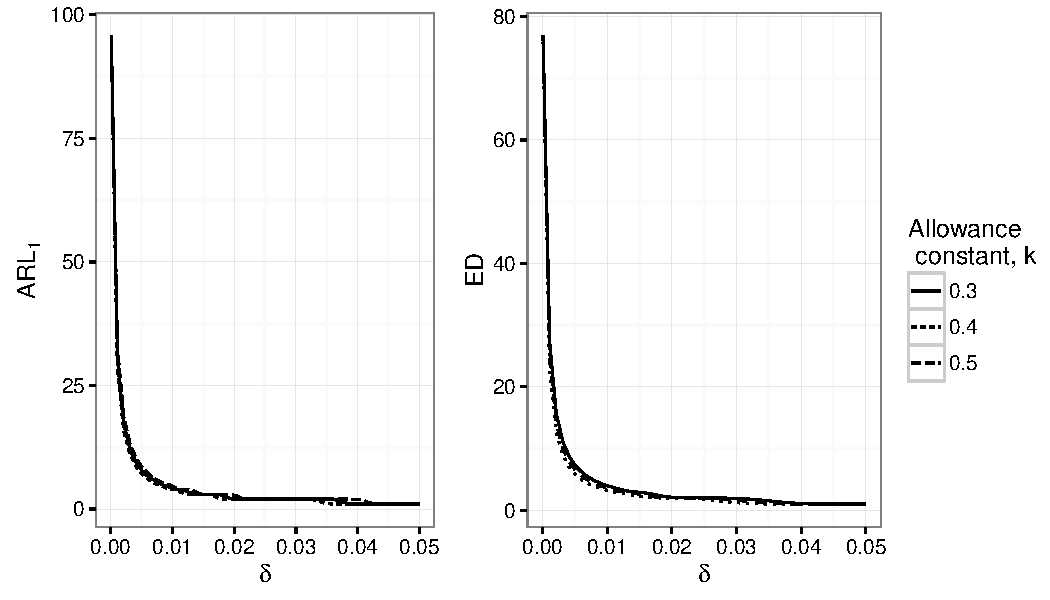
\includegraphics[width=\maxwidth]{figure/ARL1MeanCase1-1} \caption[Out-of-control ARL and ED for the MCUSUM chart of Scenario 1 - changes in the mean of all variables of lane one]{Out-of-control ARL and ED for the MCUSUM chart of Scenario 1 - changes in the mean of all variables of lane one.}\label{fig:ARL1MeanCase1}
\end{figure}


\end{knitrout}

\begin{knitrout}
\definecolor{shadecolor}{rgb}{0.969, 0.969, 0.969}\color{fgcolor}\begin{kframe}
\begin{alltt}
\hlstd{ARL1sigma} \hlkwb{<-} \hlkwd{do.call}\hlstd{(}\hlstr{"rbind"}\hlstd{,ARL1Sigma.case1)}
\hlkwd{colnames}\hlstd{(ARL1sigma)} \hlkwb{<-}  \hlstd{changeVectorSigma.case1}

\hlstd{EDsigma} \hlkwb{<-} \hlkwd{do.call}\hlstd{(}\hlstr{"rbind"}\hlstd{, EDSigma.case1)}
\hlkwd{colnames}\hlstd{(EDsigma)} \hlkwb{<-}  \hlstd{changeVectorSigma.case1}
\hlstd{EDsigma}\hlkwb{<-} \hlkwd{round}\hlstd{(EDsigma,}\hlnum{2}\hlstd{)}
\hlcom{#xtable(ARL1sigma)}
\hlcom{#xtable(EDsigma)}
\hlcom{# xtable code above generates the tables and was then pasted/manipulated into the printed format in the thesis. }
\end{alltt}
\end{kframe}
\end{knitrout}
In Table \ref{LongTable1} we have the simulated ARL$_1$ and ED for persistent changes in the covariance matrix. For small changes in the variance of the covariance matrix it takes a long time, on average, to discover the change. As $\Delta$ grows the MCUSUM chart for the covariance matrix detects changes faster. For this specific scenario and shifts the allowance constant $k$ seem to be optimal at $0.5$. The ARL$_1$ and ED is smaller for a allowance constant equal to $0.5$ compared to a allowance constant equal to $0.3$ or $0.4$.
\begin{table}[ht]
\centering
\caption{Scenario 1. MCUSUM simulated out-of-control ARL and ED for changes in covariance matrix. Each cell is on the following form: ARL$_1$ (ED). The ARL$_0$ is equal to 100. $10^5$ replications was used in this simulation study.\label{LongTable1}}
\begin{tabular}{lccccc}
\toprule
& \multicolumn{5}{c}{$\Delta$} \\ \cmidrule(r){2-6}
$k$ & 0.01 & 0.1325 & 0.255 & 0.3775 & 0.5 \\[0.1cm]
\midrule
\rowcolor[gray]{.9}  0.3 & 92.84 (72.00) & 59.59 (43.69) & 30.55 (23.19) & 18.84 (11.49) & 13.72 (6.84) \\[0.1cm]
\midrule
\rowcolor[gray]{.85}  0.4 & 94.18 (72.23) &  57.54 (45.90) & 25.71 (21.32) & 14.49 (8.97) & 10.87 (4.44) \\[0.1cm]
\midrule
\rowcolor[gray]{.9}  0.5 & 87.16 (76.87) & 48.35 (39.75) & 18.11 (12.80) & 10.44 (3.47) & 7.85 (1.10) \\[0.1cm] 
\bottomrule
\end{tabular}
\end{table}

\subsubsection{Scenario 2 - The error rate of lane 1 shows increasingly poor behaviour}
\begin{knitrout}
\definecolor{shadecolor}{rgb}{0.969, 0.969, 0.969}\color{fgcolor}\begin{kframe}
\begin{alltt}
\hlstd{ChangeMeanFun}\hlkwb{<-} \hlkwa{function}\hlstd{(}\hlkwc{mu0}\hlstd{,}\hlkwc{x}\hlstd{) \{}
  \hlstd{mu0} \hlopt{+} \hlkwd{c}\hlstd{(}\hlkwd{rep}\hlstd{(}\hlkwd{c}\hlstd{(}\hlnum{0}\hlstd{,}\hlnum{0}\hlstd{,x),}\hlnum{2}\hlstd{),}\hlkwd{rep}\hlstd{(}\hlnum{0}\hlstd{,}\hlkwd{length}\hlstd{(mu0)}\hlopt{-}\hlnum{6}\hlstd{))}
\hlstd{\}}

\hlstd{HotellingChange}\hlkwb{<-} \hlkwa{function}\hlstd{(}\hlkwc{i}\hlstd{)\{}
  \hlstd{data} \hlkwb{<-} \hlstd{MASS}\hlopt{::}\hlkwd{mvrnorm}\hlstd{(}\hlkwc{n}\hlstd{=}\hlnum{500}\hlstd{,} \hlkwc{mu}\hlstd{=}\hlkwd{ChangeMeanFun}\hlstd{(}\hlkwc{mu0} \hlstd{= mu0,} \hlkwc{x}\hlstd{=i),} \hlkwc{Sigma}\hlstd{=Sigma0)}
  \hlstd{Hotellings} \hlkwb{<-} \hlkwd{apply}\hlstd{(data,}\hlnum{1}\hlstd{,} \hlkwa{function}\hlstd{(}\hlkwc{j}\hlstd{)} \hlkwd{HotellingT2}\hlstd{(}\hlkwc{x_new}\hlstd{=j,} \hlkwc{mu0}\hlstd{=mu0,} \hlkwc{Sigma0}\hlstd{=Sigma0))}
  \hlstd{FirstAbove} \hlkwb{<-} \hlkwd{which}\hlstd{(Hotellings}\hlopt{>}\hlstd{QuantileHot)} \hlopt \hlkwd{first}\hlstd{()}

  \hlkwa{if} \hlstd{(}\hlkwd{is.na}\hlstd{(FirstAbove)}\hlopt{==}\hlnum{TRUE}\hlstd{)}
  \hlstd{\{}
    \hlstd{FirstAbove} \hlkwb{<-} \hlnum{500}
  \hlstd{\}}
  \hlkwd{return}\hlstd{(FirstAbove)}
\hlstd{\}}

\hlstd{exChange}\hlkwb{<-} \hlstd{changeVector.case2[}\hlkwd{c}\hlstd{(}\hlnum{1}\hlstd{,}\hlnum{3}\hlstd{,}\hlnum{5}\hlstd{,}\hlnum{8}\hlstd{,}\hlnum{10}\hlstd{)]}
\hlcom{#Hot_list2 <- c()}
\hlcom{#for (i in exChange)\{}
\hlcom{#  mcuh <- replicate(1e5, HotellingChange(i=i))}
\hlcom{#  Hot_list2 <- c(Hot_list2, mean(mcuh))}
\hlcom{#\}}
\hlcom{#save(Hot_list2, file="../Data/Scenario2Hotelling.Rdata")}
\hlkwd{load}\hlstd{(}\hlstr{"../Data/Scenario2Hotelling.Rdata"}\hlstd{)}
\end{alltt}
\end{kframe}
\end{knitrout}
In this scenario we would like to investigate how the charts behave in a situation where only two variables in a lane is effected by some unknown change. In this case we assume that $\delta_1=\delta_2=0$ and $\delta_3>0$. This implies that the error rate increase on average, for lane 1 quality measurements. In the case of changes in the covariance matrix, we assume that the variance will increase and that covariance is held constant. All elements in the matrix $\Delta_1$ are zero except for the third and sixth diagonal element. In Figure \ref{fig:ARL1meanCase2} we can see the ARL$_1$ and ED for the mean in scenario 2. Note that the values of $\delta$ are larger compared to scenario 1. In comparison to scenario 1, it takes a relatively large $\delta$ to discover a change in the error rate variables of lane 1. Hotelling's $T^2$ statistic did not show any indication of a change, the smallest out-of-control ARL for all $\delta$ was equal to $500$.

In table \ref{LongTable2} the results for the ARL$_1$ and ED for simulated changes in the covariance matrix. Here, the value of the allowance constant is seen to have a impact on detecting changes in variance structure of the covariance matrix. The optimal choice of $k$ is equal to $0.5$ for this specific scenario and size of $\Delta$. 

In Table \ref{OffsetTable} we can see the average offset of the change-point estimation procedure for scenario 1 and 2. For increasing values of $\delta$ the estimation procedure becomes more accurate, on average. For small values of $\delta$ we overestimate the change-point. For large values of $\delta$ we start to underestimate the change-point. It should be noted that in cases of large and small $\delta$ we have a very unbalanced sample. 

\begin{knitrout}
\definecolor{shadecolor}{rgb}{0.969, 0.969, 0.969}\color{fgcolor}\begin{kframe}
\begin{alltt}
\hlstd{ggplot.tmp} \hlkwb{<-} \hlkwd{do.call}\hlstd{(}\hlstr{"cbind"}\hlstd{,ARL1.case2)} \hlopt \hlkwd{as.data.frame}\hlstd{()}
\hlstd{ggplot.tmp}\hlopt{$}\hlstd{x} \hlkwb{<-} \hlstd{changeVector.case2}
\hlkwd{colnames}\hlstd{(ggplot.tmp)} \hlkwb{<-} \hlkwd{c}\hlstd{(}\hlkwd{paste0}\hlstd{(}\hlstr{"k"}\hlstd{,}\hlkwd{c}\hlstd{(}\hlnum{0.3}\hlstd{,}\hlnum{0.4}\hlstd{,}\hlnum{0.5}\hlstd{)),} \hlstr{"x"}\hlstd{)}
\hlstd{p1} \hlkwb{<-} \hlkwd{ggplot}\hlstd{(ggplot.tmp)}\hlopt{+}
  \hlkwd{geom_line}\hlstd{(}\hlkwd{aes}\hlstd{(}\hlkwc{y}\hlstd{=k0.3,}\hlkwc{x}\hlstd{=x,} \hlkwc{linetype}\hlstd{=}\hlstr{"solid"}\hlstd{))} \hlopt{+}
  \hlkwd{geom_line}\hlstd{(}\hlkwd{aes}\hlstd{(}\hlkwc{y}\hlstd{=k0.4,}\hlkwc{x}\hlstd{=x,} \hlkwc{linetype}\hlstd{=}\hlstr{"dashed"}\hlstd{))} \hlopt{+}
  \hlkwd{geom_line}\hlstd{(}\hlkwd{aes}\hlstd{(}\hlkwc{y}\hlstd{=k0.5,}\hlkwc{x}\hlstd{=x,} \hlkwc{linetype}\hlstd{=}\hlstr{"dotdash"}\hlstd{))} \hlopt{+}
  \hlkwd{ylab}\hlstd{(}\hlkwd{expression}\hlstd{(ARL[}\hlnum{1}\hlstd{]))} \hlopt{+}
  \hlkwd{xlab}\hlstd{(}\hlkwd{expression}\hlstd{(delta))} \hlopt{+}
  \hlkwd{scale_linetype}\hlstd{(}\hlstr{"Allowance \textbackslash{}n constant"}\hlstd{,} \hlkwc{labels}\hlstd{=}\hlkwd{paste0}\hlstd{(}\hlstr{"0."}\hlstd{,}\hlnum{3}\hlopt{:}\hlnum{5}\hlstd{))} \hlopt{+}
  \hlkwd{theme_bw}\hlstd{()} \hlopt{+}
  \hlkwd{theme}\hlstd{(}\hlkwc{legend.position}\hlstd{=}\hlstr{"right"}\hlstd{)}


\hlstd{ggplot.tmp} \hlkwb{<-} \hlkwd{do.call}\hlstd{(}\hlstr{"cbind"}\hlstd{,ED.case2)} \hlopt \hlkwd{as.data.frame}\hlstd{()}
\hlstd{ggplot.tmp}\hlopt{$}\hlstd{x} \hlkwb{<-} \hlstd{changeVector.case2}
\hlkwd{colnames}\hlstd{(ggplot.tmp)} \hlkwb{<-} \hlkwd{c}\hlstd{(}\hlkwd{paste0}\hlstd{(}\hlstr{"k"}\hlstd{,}\hlkwd{c}\hlstd{(}\hlnum{0.3}\hlstd{,}\hlnum{0.4}\hlstd{,}\hlnum{0.5}\hlstd{)),} \hlstr{"x"}\hlstd{)}

\hlstd{p2} \hlkwb{<-} \hlkwd{ggplot}\hlstd{(ggplot.tmp)} \hlopt{+}
  \hlkwd{geom_line}\hlstd{(}\hlkwd{aes}\hlstd{(}\hlkwc{y}\hlstd{=k0.3,}\hlkwc{x}\hlstd{=x),} \hlkwc{linetype}\hlstd{=}\hlnum{1}\hlstd{)} \hlopt{+}
  \hlkwd{geom_line}\hlstd{(}\hlkwd{aes}\hlstd{(}\hlkwc{y}\hlstd{=k0.4,}\hlkwc{x}\hlstd{=x),} \hlkwc{linetype}\hlstd{=}\hlnum{2}\hlstd{)} \hlopt{+}
  \hlkwd{geom_line}\hlstd{(}\hlkwd{aes}\hlstd{(}\hlkwc{y}\hlstd{=k0.5,}\hlkwc{x}\hlstd{=x),} \hlkwc{linetype}\hlstd{=}\hlnum{3}\hlstd{)} \hlopt{+}
  \hlkwd{theme_bw}\hlstd{()} \hlopt{+}
  \hlkwd{ylab}\hlstd{(}\hlstr{"ED"}\hlstd{)} \hlopt{+}
  \hlkwd{xlab}\hlstd{(}\hlkwd{expression}\hlstd{(delta))} \hlopt{+}
  \hlkwd{theme}\hlstd{(}\hlkwc{legend.position}\hlstd{=}\hlstr{"none"}\hlstd{)}
\hlstd{p3} \hlkwb{<-} \hlkwd{get_legend}\hlstd{(p1)}
\hlstd{p1} \hlkwb{<-} \hlstd{p1} \hlopt{+} \hlkwd{theme}\hlstd{(}\hlkwc{legend.position}\hlstd{=}\hlstr{"none"}\hlstd{)}

\hlkwd{grid.arrange}\hlstd{(p1,p2,p3,} \hlkwc{ncol}\hlstd{=}\hlnum{3}\hlstd{,} \hlkwc{widths}\hlstd{=}\hlkwd{c}\hlstd{(}\hlnum{2.3}\hlstd{,} \hlnum{2.3}\hlstd{,} \hlnum{0.8}\hlstd{))}
\end{alltt}
\end{kframe}\begin{figure}
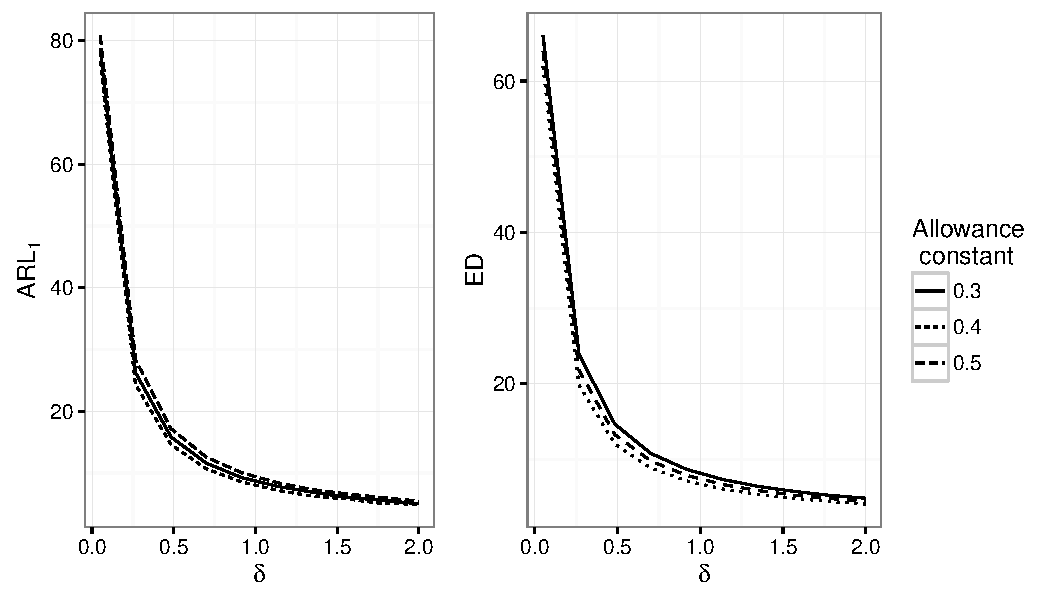
\includegraphics[width=\maxwidth]{figure/ARL1meanCase2-1} \caption[Out-of-control ARL simulations of Scenario 2 - changes in the mean of the error rate of lane one]{Out-of-control ARL simulations of Scenario 2 - changes in the mean of the error rate of lane one.}\label{fig:ARL1meanCase2}
\end{figure}


\end{knitrout}

\begin{knitrout}
\definecolor{shadecolor}{rgb}{0.969, 0.969, 0.969}\color{fgcolor}\begin{kframe}
\begin{alltt}
\hlstd{ARL1sigma} \hlkwb{<-} \hlkwd{do.call}\hlstd{(}\hlstr{"rbind"}\hlstd{,ARL1Sigma.case2)}
\hlkwd{colnames}\hlstd{(ARL1sigma)} \hlkwb{<-}  \hlstd{changeVectorSigma.case2}

\hlstd{EDsigma} \hlkwb{<-} \hlkwd{do.call}\hlstd{(}\hlstr{"rbind"}\hlstd{, EDSigma.case2)}
\hlkwd{colnames}\hlstd{(EDsigma)} \hlkwb{<-}  \hlstd{changeVectorSigma.case2}
\hlstd{EDsigma}\hlkwb{<-} \hlkwd{round}\hlstd{(EDsigma,}\hlnum{2}\hlstd{)}

\hlcom{#xtable(ARL1sigma)}
\hlcom{#xtable(EDsigma)}
\end{alltt}
\end{kframe}
\end{knitrout}

\begin{table}[ht]
\centering
\caption{Scenario 2. MCUSUM simulated out-of-control ARL and ED for changes in covariance matrix. Each cell is on the following form: ARL$_1$ (ED). The ARL$_0$ is equal to 100. $10^5$ replications was used in this simulation study.\label{LongTable2}}
\begin{tabular}{lccccc}
\toprule
& \multicolumn{5}{c}{$\Delta$} \\ \cmidrule(r){2-6}
$k$ & 0.05 & 0.6625 & 1.275 & 1.8875 & 2.5 \\[0.1cm] 
\midrule
\rowcolor[gray]{.9} 0.3 & 94.45 (74.05) & 70.15 (51.24) & 49.53 (34.93) & 35.46 (23.63) & 26.87 (16.88) \\[0.2cm]
\midrule
\rowcolor[gray]{.85}  0.4 & 95.46 (73.17) & 68.24 (49.39) & 46.28 (31.53) & 30.98 (19.90) & 22.21 (12.89) \\[0.2cm] 
\midrule
\rowcolor[gray]{.9}  0.5 & 88.29 (66.32) & 58.54 (42.01) & 37.56 (23.46) & 22.31 (12.33) & 15.44 (6.60) \\[0.2cm] 
\bottomrule
\end{tabular}
\end{table}

\begin{table}[ht]
\centering
\caption{Table containing $\bar{D}$ for both scenarios. Each cell is listed in the following way: $\bar{D}\; (\text{Number out-of-control obs.})$ 20 in control observations was used.\label{OffsetTable}}
\begin{tabular}{lcccccccccc}
\toprule
\textbf{Scenario 1} & \multicolumn{10}{c}{$\delta$} \\ \cmidrule(r){2-11} 
 & 0.0001 & 0.0052 & 0.0103 & 0.0164 & 0.0215 & 0.0276 & 0.0327 & 0.0388 & 0.0439 & 0.0500 \\  \\[0.1cm]
\rowcolor[gray]{.9}  $\bar{D}$ & 42.63 & 6.43 & 0.29 & -0.06 & -0.21 & -0.24 & -0.41 & -0.88 & -1.77 & -1.63 \\[0.1cm]
\midrule
\textbf{Scenario 2} & \multicolumn{10}{c}{$\delta$} \\ \cmidrule(r){2-11} 
 & 0.05 & 0.27 & 0.48 & 0.70 & 0.92 & 1.13 & 1.35 & 1.57 & 1.78 & 2.00 \\[0.1cm] 
\rowcolor[gray]{.85}  $\bar{D}$ & 41.65 & 5.60 & 0.20 & -0.04 & -0.13 & -0.17 & -0.31 & -0.75 & -1.64 & -1.53 \\
\bottomrule
\end{tabular}
\end{table}
% \subsection{Robustness (optional section)}
% \begin{enumerate}
% \item What happens under the t-distribution or maybe something skew? 
% \item What happens when the mean and/or covariance matrix is wrongly estiamted? How does this effect control limits etc? 
% \end{enumerate}
\bibliography{REFERENCES.bib}
\end{document}
